\documentclass[runningheads]{llncs}
\usepackage{graphicx}
\usepackage{float}
\usepackage[text={150mm,220mm},centering,nohead]{geometry}
\pagestyle{empty} 
\begin{document}    
\title{\large{CSCI933-Machine Learning and Application}
\author{}
\institute{}
\maketitle
\vspace{-1cm}
%-----------Please Do NOT change the content above.-----------------

%---------------------------------------------------------------------------------------------------------------------------------

%-----------Please write the project information here.---------------

\begin{center}
\Large{\textbf{The Classification and Prediction of Pima-Indians-Diabetes.data}} \\ % Please write your project tile in here
\vspace{0.2cm}
\large{\emph{Group Members: ZijiaHe, ChangXu, HongyiHuang, WangzhihuiMei}} \\%Please write names of your group members as well as the group number in here
\vspace{0.3cm}  
\end{center}

%-----------Please write the content of your research proposal from here.---------------

\section{Introduction}
The data set we used was collected by the 
National Institute of Diabetes and Digestive and Kidney Diseases 
from a group of women and Pima Indian descendants at least 21 years old. The goal is to use patient information to predict whether a patient has diabetes.
There are 8 features:\\
1. Number of times pregnant\\
2. Plasma glucose concentration a 2 hours in an oral glucose tolerance test\\
3. Diastolic blood pressure (mm Hg)\\
4. 2-Hour serum insulin (mu U/ml)\\
5. Triceps skin fold thickness (mm)\\
6. Body mass index (weight in kg/$(height in m)^2$)\\
7. Diabetes pedigree function\\
8. Age (years)\\
And 1 label (response variable). These data are collected from actual patients and represent a task, 
usually performed by a human doctor, with the purpose of identifying the patients most likely to have
diabetes in order to propose preventive measures. \\
Next, we conducted some comparative studies on these data, we can get a table:\\
\begin{figure}[H]
    \centering
    
\includegraphics[scale=0.6]{1.PNG}  
\end{figure}

\begin{figure}[H]
    \centering
    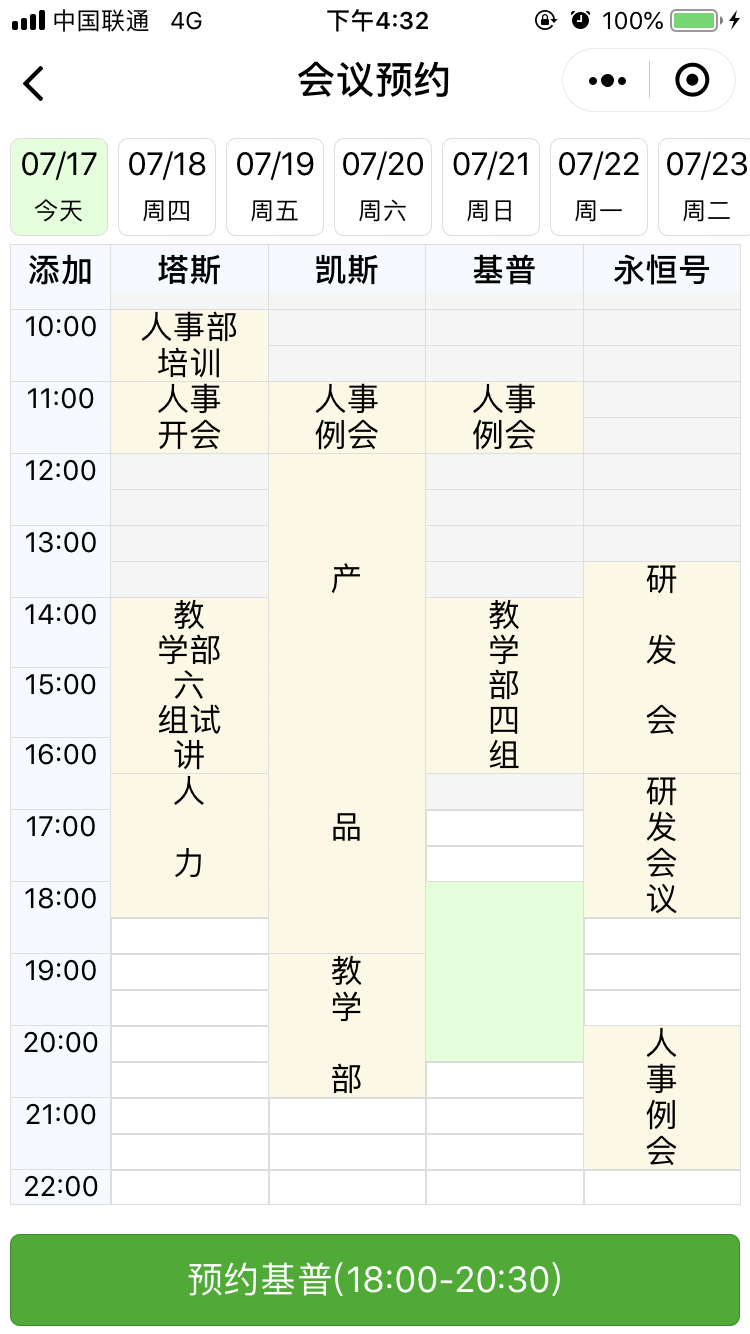
\includegraphics[scale=0.6]{2.PNG}  
\end{figure}


There are some problems from tables above:
The lowest blood glucose, blood pressure, skin thickness, insulin, BMI are all 0. 
This seems suspicious because these physical quantities cannot be 0 (for living people). 
Therefore, this has told us that we need to estimate these five columns. 
The scope of other variables seems to be reasonable.\\
However,there are still some informations from the dataset:
Higher blood sugar correlates with a result of 1, which means
 that the patient has diabetes. Age also seems to be related to
  diabetes: younger patients have a lower risk of diabetes.
\clearpage



\begin{flushleft}
\huge{\textbf{Appendix}}
\end{flushleft}
\begin{center}
\Large{\textbf{A web portal for online purchase services}} \\*[0.1cm]%Please write names of the project title in here
\large{\emph{Group Members (5): ZijiaHe, ChangXu, HongyiHuang, ZhanpingZhou}} %Please write names of your group members as well as the group number in here
\end{center}
%----------------------------------------------------------------------------------------------------------------------------


%-----------Please write the content of your appendix (diagrams, figures, tables, etc) from here.---------------
\noindent 

\end{document}

